\documentclass{bdrvntu}

\usepackage{tabularx}    % для формування таблиць
\usepackage{amsmath}     % текст у формулах
\usepackage{amssymb}     %
\usepackage{minted}      % лістинги коду
\usepackage{listings}    %
\usepackage{lstfiracode} %
\usepackage{nicefrac}    % для дробів

                                               
%!TEX root = ../bdr.tex
% основні параметри які можна змінити/задати в документі класу bdrvntu

%% навчальний заклад. По замовчанню "Вінницький національний технічний унверситет", але можна змінити на інший командою \educational{}, як наприклад:
%\educational{Національний університет <<Львівська політехніка>>}
%% навчальний заклад абревіатурою. По замовчанню "ВНТУ", але можна змінити на іншу командою \educationalabbr{}, як наприклад:
%\educationalabbr{НУЛП}
%% місто. По замовчанню "Вінниця", але можна змінити на інше командою \city{}, як наприклад:
%\city{Львів}
%% факультет. По замовчанню "комп'терних систем і автоматики", але можна змінити на інший командою \faculty{}, як наприклад:
\faculty{інтелектуальних інформаційних технологій та автоматизації}
%% кафедра. По замовчанню "автоматизації та інтелектуальних інформаційних технологій", але можна змінити на іншу командою \department{}, як наприклад:
%\department{метрології та промислової автоматики}
%% кафедра абревіатурою. По замовчанню "АІІТ", але можна змінити на іншу командою \departmentabbr{}, як наприклад:
%\departmentabbr{МПА}
%% тема роботи. Значення по замочанню не присвоєне, необхідно обов'язково задавати.
\title{вдосконалення системи управління якості програмного забезпечення}

%% студент
%% курсу. Значення по замочанню не присвоєне, необхідно обов'язково задавати.
\course{IV}
%% групи. Значення по замочанню не присвоєне, необхідно обов'язково задавати.
\group{АКІТ-20б}
%% спеціальності. Значення по замочанню не присвоєне, необхідно обов'язково задавати.
\speciality{151 -- Автоматизація та комп’ютерно-інтегровані технології}
%% ім'я. Значення по замочанню не присвоєне, необхідно обов'язково задавати.
\author{Петровський Д. Ю.}
%% ім'я в родовому відмінку. Фігурує в індивідуальному завданні. Значення по замочанню не присвоєне, необхідно обов'язково задавати.
\gcauthor{Петровському Дмитру Юрійовичу}
     
%% керівник
%% ім'я. Значення по замочанню не присвоєне, необхідно обов'язково задавати.
\leader{Овчинников К. В.}
%% науковий ступінь керівника. Значення по замочанню не присвоєне, необхідно обов'язково задавати.
\degree{к.т.н.}
%% педагогічне звання. Значення по замочанню не присвоєне, необхідно обов'язково задавати.
\position{доцент}
%% передбачається, що керівник з кафедри здобувача. Абревіатура для них однакова і задається командою \departmentabbr{}, що описани вище.

%% рецензент
%% ім'я. Значення по замочанню не присвоєне, необхідно обов'язково задавати.
\reviewer{Тарновський М. Г.}
% науковий ступінь рецензента. Значення по замочанню не присвоєне, необхідно обов'язково задавати.
\reviewerdegree{к.т.н.}
%% педагогічне звання. Значення по замочанню не присвоєне, необхідно обов'язково задавати.
\reviewerposition{доцент}
%% кафедра рецензента абревіатурою. Значення по замочанню не присвоєне, необхідно обов'язково задавати. 
\rdepartmentabbr{КСУ}

%% рік видання
%% рік видання проставляється автоматично в момент останньої компіляції, але якщо потрібно його можна змінити командою \annum{}, як наприклад:
% \annum{2021}

%% індивідуальне завдання
%% галузь знань. Значення по замочанню не присвоєне, необхідно обов'язково задавати.
\branchofknowledge{автоматизація та приладобудування} 
%% освітня програма. Значення по замочанню не присвоєне, необхідно обов'язково задавати.
\educationalprogram{автоматизація та комп’ютерно-інтегровані технології}

%% для креслеників
%% перевірив (нормоконтроль). Значення по замочанню не присвоєне, необхідно обов'язково задавати.
\controller{Овчинников К. В.}
%% затвердив. Значення по замочанню не присвоєне, необхідно обов'язково задавати.
\approver{Бісікало О. В.} 

%% статус очільника кафедри. Значення по замовчанню "Завідувач кафедри"
\dpheaderstatus{в.о. зав. кафедри}

\typeofwork{Бакалаврська дипломна робота}
\acstypeofwork{бакалаврську дипломну роботу}







  % варіативні значення 

\hypersetup{colorlinks,  % кольорові(сині) посилання по тексту
            allcolors=black,
            urlcolor=blue,
            pageanchor=false}
                    
                       
\begin{document}
\maketitle                           % титульний аркуш
%%!TEX root = ../bdr.tex
\begin{assignment}%
{}%наказ по університету
{}%строк подання роботи студентом
{}%вихідні дані до роботи
{}%зміст розрахунково-пояснювальної записки
{}%перелік графічного матеріалу
{}%консультанти розділів роботи
{}%дата видачі завдання
{}%календарний план
\end{assignment}    % порожнє індивідуальне завдання 
%!TEX root = ../bdr.tex
\begin{assignment}%
%наказ по університету
{\guillemotleft9\guillemotright~березня 2021 року №~65}
%
%строк подання роботи студентом
{07.06.2021}
%
%вихідні дані до роботи
{\begin{itemize}
\item {діапазон вимірювання тиску – не менше 70 МПа;}
\item {діапазон вимірювання переміщення – не менше 250 мм;}
\item {інтерфейс передавання даних – RS-485.}
\end{itemize}}
%
%зміст розрахунково-пояснювальної записки
{Провести огляд існуючих систем та засобів для визначення придатності до використання колісних пар залізничних вагонів, запропонувати структуру мікропроцесорної системи вихідного контролю пресових з’єднань колісних пар залізничних вагонів, розробити алгоритм роботи та програмне забезпечення мікропроцесорної системи вихідного контролю пресових з’єднань колісних пар залізничних вагонів}
%
%перелік графічного матеріалу
{Мікропроцесорна система вихідного контролю пресових з’єднань колісних пар заліз-ничних вагонів, схема електрична структурна; Мікропроцесорна система вихідно-го контролю пресових з’єднань колісних пар залізничних вагонів, схема електри-чна функціональна; Мікропроцесорна система вихідного контролю пресових з’єднань колісних пар залізничних вагонів, схема роботи програми}
%
%консультанти розділів роботи
{\begin{tabular}{|p{1.8cm}|p{8.4cm}|p{2.5cm}|p{2.5cm}|}\hline
  \multirow{2}{*}{Розділ} & \multirow{2}{*}{\parbox{8.4cm}{\centering{Прізвище, ініціали та посада\\ консультанта}}} & \multicolumn{2}{c|}{Підпис, дата} \\ \cline{3-4}
  & & завдання видав & завдання прийняв \\ \hline
  1 & ??? &  &  \\ \hline 
  2 & ??? &  &  \\ \hline
  3 & ??? &  &  \\ \hline
  4 & ??? &  &  \\ \hline
\end{tabular}}
%
%дата видачі завдання
{03.02.2021}
%
%календарний план
{\begin{tabular}{|p{0.8cm}|p{9.0cm}|p{3.4cm}|p{2.0cm}|}\hline
  № з/п & Назва етапів бакалаврської дипломної роботи & Строк виконання & Примітка \\ \hline
  1 & Огляд існуючих систем та засобів визначення придатності  пресових з’єднань & 01.02.2021 26.02.2021 &  \\ \hline 
  2 & Огляд методів вимірювання надлишкового тиску та переміщення &  &  \\ \hline
  3 & Розробка схеми функціональної мікропроцесорної системи &  &  \\ \hline
  4 & Вибір компонентів для використання в складі мікропроцесорної  системи &  &  \\ \hline
\end{tabular}}
\end{assignment}           % індивідуальне завдання заповнене майже повністю 
%%!TEX root = ../bdr.tex
%two page annotations
\frontmatter
\chapter*{\abstractname}% \chapter*{} - заголовок розділу без номера 
\thispagestyle{empty}

Поданий документ складається зі вступу, двох розділів, висновків, переліку використаних джерел
(\total{citnum} бібліографічних посилань) та додатків. Загальний обсяг роботи (\total{page} сторінки) містить
рисунків \total{figures}, таблиць \total{tables}.

Шаблон створено для ознайомлення з основними можливостями видавничої системи {\LaTeX} в цілому та можливостями 
класу документу \verb|bdrvntu| зокрема. Автори в доступній формі спробували донести до читача основні принципи
створення документу.

Ключові слова: видавнича система, {\TeX}, {\LaTeX}, бакалавр, кваліфікаційна робота.

\chapter*{Annotation}
\thispagestyle{empty}

The submitted document consists of an introduction, two sections, conclusions,
list of used sources (\total{citnum} bibliographic references) and appendices.
The total volume of work (\total{page} pages) contains figures \total{figures}, tables \total{tables}.

The template was created to get acquainted with the main features of
the old {\LaTeX} system as a whole and the capabilities of the bdrvntu document class
in particular. The authors tried to convey the main points to the reader in an accessible form
principles of document creation.

Key words: publishing system, {\TeX}, {\LaTeX}, bachelor, qualification
valuable work.

\newpage
\mainmatter      % анотації кожна на окремій сторінці
%!TEX root = ../bdr.tex
%same page annotations
\frontmatter
\chapter*{Анотація}% \chapter*{} - заголовок розділу без номера 
\thispagestyle{empty}

Поданий документ складається зі вступу, двох розділів, висновків, переліку використаних джерел
(\total{citnum} бібліографічних посилань) та додатків. Загальний обсяг роботи (\total{page} сторінки) містить
рисунків \totfig{}, таблиць \tottab{}.

Шаблон створено для ознайомлення з основними можливостями видавничої системи {\LaTeX} в цілому та можливостями 
класу документу \verb|bdrvntu| зокрема. Автори в доступній формі спробували донести до читача основні принципи
створення документу.

Ключові слова: видавнича система, {\TeX}, {\LaTeX}, бакалавр, кваліфікаційна робота.

\vspace{6ex}

{\let\clearpage\relax\chapter*{Annotation}}

The submitted document consists of an introduction, two sections, conclusions,
list of used sources (\total{citnum} bibliographic references) and appendices.
The total volume of work (\total{page} pages) contains figures \totfig{}, tables \tottab{}.

The template was created to get acquainted with the main features of
the old {\LaTeX} system as a whole and the capabilities of the bdrvntu document class
in particular. The authors tried to convey the main points to the reader in an accessible form
principles of document creation.

Key words: publishing system, {\TeX}, {\LaTeX}, bachelor, qualification
valuable work.

\newpage
\mainmatter       % дві анотації на одній сторінці
\tableofcontents                     % зміст                     
%!TEX root = ../bdr.tex
\chapter*{Вступ}

Пояснювальна записка до бакалаврської кваліфікаційної роботи є складним та великим за обсягом документом, який містить
багато iлюстрацiй, таблиць, математичних формул, посилань на структурнi частини роботи, формули та джерела у списку 
лiтератури. Протягом роботи над пояснювальною запискою автор повинен постiйно редагувати свiй генiальний текст,
часто термiново. В таких умовах важко витримувати сталою загальну структуру роботи, слідкувати за тим, щоб посилання
на всі структурні частини тексту, рисунки, таблиці, літературні джерела, тощо залишались коректними. І це далеко не все,
що може <<поїхати>> в тексті при редагуванні. Допомогти в цьому може система \LaTeX, одна з найпотужнiших i найефективнiших 
сучасних систем підготовки документів, що ґрунтується на системi комп’ютерного верстування \TeX \cite{latexctan}.

Клас {\LaTeX} {\verb|bdrvntu|} призначений для оформлення пояснювальної записки до бакалаврської кваліфікаційої роботи згiдно вимог,
що висуваються до такого роду робіт у Вінницькому національному технічному університеті а саме:

\begin{itemize}
\item оформлення титульної сторінки;
\item оформлення сторінки індивідуального завдання;
\item оформлення заголовків, розділів, підрозділів та додатків;
\item нумерація сторінок, рисунків, таблиць, формул, тощо;
\item оформлення списку використаних джерел та ін.
\end{itemize} 

Як i будь-який клас документа, він має допомогти автору роботи зосередитися на написаннi власне тексту i використовувати 
логiчну розмiтку тексту замiсть його безпосереднього оформлення.             % вступ
%!TEX root = ../bdr.tex
\chapter{Верстування текстової частини роботи}
А це просто текст...

Порожній рядок означає, що це був абзац

%\textbf{Lorem Ipsum is simply dummyl}  text of the printing and typesetting industry. Lorem Ipsum has been the industry's standard dummy text ever since the 1500s, when an unknown printer took a galley of type and scrambled it to make a type specimen book. It has survived not only five centuries, but also the leap into electronic typesetting, remaining essentially unchanged. It was popularised in the 1960s with the release of Letraset sheets containing Lorem Ipsum passages, and more recently with desktop publishing software like Aldus PageMaker including versions of Lorem Ipsum. 
\lipsum[2-4]

А це ненумерований список:
\begin{itemize}
\item Зелений;
\item Жовтий;
\item Білий.
\end{itemize}

А це нумерований список:
\begin{enumerate}
\item Колір
      \begin{enumerate}
      \item Зелений;
      \item Жовтий;
      \item Білий.
      \end{enumerate}	
\item Температура
      \begin{enumerate}
      \item Теплий;
      \item Холодний.
      \end{enumerate}
\end{enumerate}
 

\section{Рисунки}

Вставка рисунків робиться дуже просто:

\begin{figure}[h]
\caption{Опис рисунку}
\end{figure}

Далі можна вставити і сам рисунок (рис. \ref{fig:tux}). Він має бути у графічному файлі ({*}.jpg, {*}.png тощо). 

\begin{figure}[h]
 \centering
\includegraphics{img/Tux.png}
 \caption{Пінгвін}
 \label{fig:tux}
\end{figure}

Рисунок можна винести і в додаток (додаток \ref{apdx:text}), \label{linkpage} а посилання на нього залишити в основній частині роботи (рис. \ref{apdxfig:tux}).
Можна вручную вставляти картинки і прописувати кожний параметр.
Параметр width визначає ширину рисунку. У цьому випадку вона дорівнюватиме ширині текста \verb|\textwidth|. Замість \verb|\textwidth| можна вказати значення від 0.1 до 1. \verb|\label| потрібна для того, щоби потім можна було послатись на цю картинку, як тут.

\begin{figure}[!htb]
 \centering
 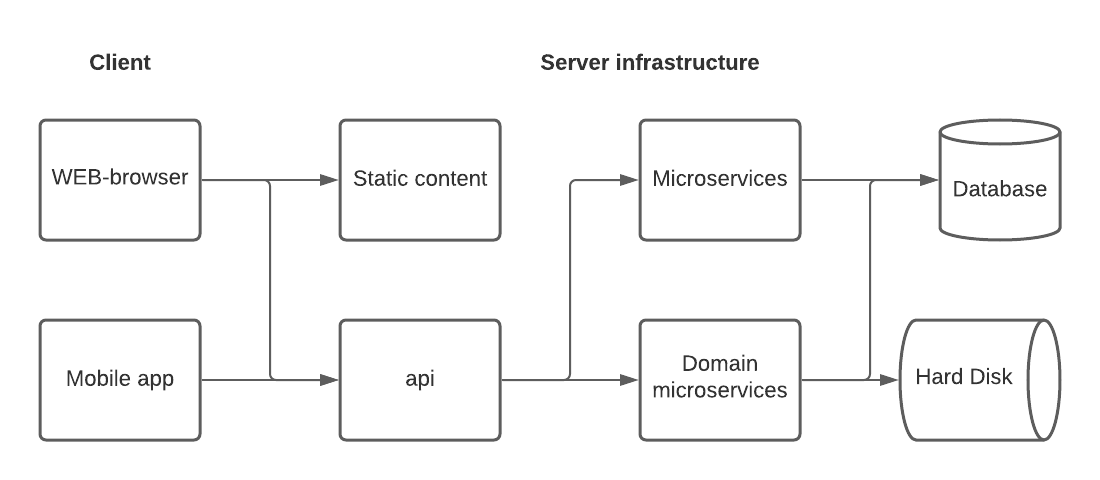
\includegraphics[width=0.8\textwidth]{img/fig1.png}
 \caption{Використовуйте Rich Text}
 \label{fig:fig1}
\end{figure}

\section{Таблиці}
Таблиці  - це складний об'єкт. Тому всі параметри треба прописувати вручну

\begin{table}[h!]
\centering
\begin{tabular}{|c|c|c|c|} 
 \hline
 Стопець1 & Стопець2 & Стопець3 & Стопець4 \\ [0.5ex] 
 \hline
 \multirow{3}{5em}{Декілька рядків} & 6 & 87837 & 787 \\ 
  &  7 & 78 & 5415 \\
   & 545 & 778 & 7507 \\
   & 545 & 18744 & 7560 \\
   & 88 & 788 & 6344 \\ [1ex] 
 \hline
\end{tabular}
\caption{Приклад роботи з таблицею}
\label{table:1}
\end{table}

\begin{table}[h]
	\caption{\label{table:2}Функціональна залежність параметрів ...}
	%\label{table:2}
	\begin{tabular}{|c|c|c|}
		\hline 
		Індекс & Показник 1 & Показник 2\tabularnewline
		\hline 
		\hline 
		1 & 2 & 3\tabularnewline
		\hline 
		4 & 5 & 6\tabularnewline
		\hline 
	\end{tabular}
\end{table}

Для табл. \ref{table:2} вже можете побачити легенду, яка на відміну від рисунків розташована зверху.

Великі таблиці можна повертати на 90 градусів:

%\begin{sidewaystable}
%	\centering{}
%	\caption{Набір компонентів.}
%	\begin{tabular}{|c|>{\raggedright}p{0.25\columnwidth}|>{\centering}p{0.15\columnwidth}|>{\centering}p{0.1\columnwidth}|}
%	\hline 
%	№ & Компонент  & Маса & К-сть\tabularnewline
%	\hline 
%	\hline 
%	1 & Компонент А & 12.8 & 100\tabularnewline
%	\hline 
%	2 & Компонент Б & 7.88 & 12\tabularnewline
%	\hline 
%	3 & Компонент В & 83.89 & 44\tabularnewline
%	\hline 
%	\end{tabular}
%\end{sidewaystable}

Більше про таблиці можна прочитати \href{https://www.overleaf.com/learn/latex/Tables}{тут}.

%\clearpage{}

\section{Формули...}

Формули, що входять до бакалврської роботи, нумерують в межах розділу. Номер формули складається з номера розділу та порядкового номера формули, розділених крапкою. Номер формули розташовують з правого боку на рівні формули в круглих дужках. По\-си\-лан\-ня в тексті на номер формули дають в дужках, наприклад, «... за формулою (\ref{eq:explan})». За необхідності вказують одиницю вимірювання, беручи її в квадратні дужки

\begin{equation}
\label{eq:explan}
I = \frac{U}{R}~[A].
\end{equation}

Числову підстановку і розрахунок виконують з нового рядка не нумеруючи. Одиницю вимірювання беруть в круглі дужки. Наприклад,

$$I = \frac{220}{100}~(\text{А}).$$

Розмірність одного й того ж параметра в межах документа має бути однаковою. Якщо формула велика, то її можна переносити в на\-ступ\-ні рядки. Перенесення виконують тільки математичними знаками, повторюючи знак на початку наступного рядка. При цьому знак мно\-жен\-ня «$\cdot$» замінюють знаком «$\times$».


\begin{align}
\label{xt:eq}
y(t) &= \frac{1}{{\rho}\,{S}\,{C_{f}}\,\sin\alpha}\Big(\ln\Big(\frac{1}{1962\,m}\Big(10\,v_0\sqrt{\rho\,S\,C_f\,\sin^3\alpha}\,\times \nonumber\\  &\times\cos\Big(\frac{3\,t\,\sqrt{218\,\rho\,S\,C_f\,\sin\alpha}}{20\,\sqrt{m}}\Big)\Big)^2\Big)\,m\Big).
\end{align}


Пояснення символів та числових коефіцієнтів наводять під формулою. Пояснення кожного символа подається з нового рядка в тій послідовності, в якій символи зустрічаються в формулі. Перший рядок пояснення починається зі слова «де» без двокрапки після нього.

\begin{equation}
T = 2\pi\sqrt{\frac{m}{k}}, 
\end{equation}

\begin{explanation}
\fitem $k$ -- коефіцієнт жорсткості пружини; 
\item $m$ -- маса тягарця.
\end{explanation}

Формула є частиною речення, тому до неї застосовують такі ж правила граматики, як і до інших членів речення. Якщо формула зна\-хо\-дить\-ся в кінці речення, то після неї ставлять крапку. 

Вставляти в текст можна формули будь-якої складності, як наприклад:

\begin{equation}
	\text{f=}\sqrt[12]{\sum\left(\beta*\xi\right)*\frac{z}{\arctan(123)}}*\top f(z)
\end{equation}


Формули з нумерацією    
\begin{equation}
    f(x)=\frac{x}{1+x^2}
\end{equation}

Ще одна формула    
\begin{equation}
    x^n + y^n = z^n
\end{equation}
    
А так прописуються формули, де нумерація не потрібна \(x^2 + y^2 = z^2\).

Другий спосіб - це вставити формулу між символам долара: $x^2 + y^2 = z^2$. 

\section{Формули без нумерації. Дроби.}
Для відтворення дробей в рядку, наприклад \(\frac{3x}{2}\), можна встановити інший стиль:
    \( \displaystyle \frac{3x}{2} \).
Це також працює і у зворотньому напрямку:
    \[ f(x)=\frac{P(x)}{Q(x)} \ \ \textrm{та}
    \ \ f(x)=\textstyle\frac{P(x)}{Q(x)} \]

\section{Інтеграли}
Інтеграл \(\int_{a}^{b} x^2 dx\) всередені тексту.
    \medskip
І той самий інтеграл між рядками:
    \[
    \int_{a}^{b} x^2 \,dx
    \]
    
Детальніше можна прочитати 
\href{https://www.overleaf.com/learn/latex/Integrals,_sums_and_limits#Integrals}{тут}.

\section{Суми і добутки}
Читати 
\href{https://www.overleaf.com/learn/latex/Integrals,_sums_and_limits#Sums_and_products}{тут}.

\section{Межі}
    
    Межа \(\lim_{x\to\infty} f(x)\) всередені тексту.
    І між рядками:
    \[
    \lim_{x\to\infty} f(x)
    \]

\section{Символи}
$\alpha A$ - грецькі,  $ \lambda; \Lambda$ - физичні величины=и, $\exists; \forall$ - логічні символм\\
За \href{https://www.overleaf.com/learn/latex/List_of_Greek_letters_and_math_symbols}{цим посиланням} можна одержати інформацію про інші символи. 
А \href{https://www.overleaf.com/learn/latex/Operators}{тут} - математичні оператори.

\section{Зноски, примітки та інш.}
У тексті зручно робити різноманітні зноски та примітки. Для цього їх достатньо встановити у необхідному місці, а форматування зробить свою потужну роботу. Ось приклад зноски, що розташується знизу \footnote{Це тест до зноски 1}. 

\section{LaTeX Wiki}
 Повне введення у LaTeX читайти \href{https://www.texlive.info/CTAN/info/lshort/russian/lshortru.pdf}{тут}.




            % перший розділ
%!TEX root = ../bdr.tex

\chapter{Створення бібліоґрафії}

У TeХ \emph{бібліографія створюється автоматично}. Для цього у необхідному місці тексту достатньо вставити команду \verb|\bibliography{bibdata}| і аргументом вказати ім'я файлу із літературними джерелами.
Цей файл повинен мати розширення \verb|*.bib| (наприклад, для цього шаблону використовується файл \emph{bibdata.bib}). 

У цьому файлі знаходиться \emph{простий невпорядкований список} записів кожен з яких
описує рівно одну публікацію (тип видання, назва, автор, рік, сторінки тощо). Редагувати цей файл можна або спеціальною програмою (наприклад, JabRef) - і це зручно, або навіть будь-яким текстовим редактором. 

Власне оформлення самої бібліографії здійснюється повністю автоматично. При цьому відбувається впорядкування, нумерація і форматувння літературних джерел згідно правил. 

У бібліографію потрапляють не всі літературні джерела із файлу \verb|*.bib|, а лише ті, на які було здійснено посилання із тексту. Це означає, що можна вести один універсальний файл (базу даних) з літературою за певною тематикою, а у статтях посилатись лише на необхідні.

\section{Посилання на літературу}

Якщо існує bib-файл і він підключений до команди ``Бібліографія'', то у тексті можна робити посилання на літературні джерела, наприклад, ось так \cite{WinNT} або так \cite{Vasylenko92, Afanasyev92} або так \cite{Makilov91, Ponomarenko86, Belousova81, Tezisy, Statia, GOST7184}.

Нумерація літератури у тексті і у бібліографії здійснюється автоматично. 

            % другий розділ
%!TEX root = ../bdr.tex
\chapter*{Висновки}

Аналіз проведений в роботі вказує на те, що сьогодні існує велика кількість стандартів та технологій покликаних підвищувати якість програмного забезпе-чення, проте якість готової продукції як і раніше залишається на достатньо низь-кому рівні. Достатньо лише того, що лише 16 \% програмних проектів розпочатих в попередніх роках завершились з дотриманням графіку та перейшли у фазу заве-ршеного програмного продукту.

Очевидно, що існуючі підходи при всій своїй повноті та рівні автоматизації не здатні забезпечити достатній рівень якості ПЗ. Аналіз показав, що не малу час-тину контролю для забезпечення рівня якості необхідно проводити на ранніх ета-пах життєвого циклу програмного забезпечення.

В результаті дослідження були визначені метрики якості, та визначена їх ефективність. Обраховані граничні значенні та діапазони зміни спираючись на дані проведених досліджень. Серед найбільш ефективних метрик якості придат-них до застосування на ранніх етапах життєвого циклу ПЗ були обрані: метрика звертання до глобальних змінних, кількість виявлених помилок при інспектуван-ні, цикломатична складність, відносна гранична складність програми. Результати досліджень показують, що на рівень якості впливають не тільки метрики з широ-ким діапазоном зміни значень і нехтувати менш значущими метриками не доціль-но.
             % висновки
%!TEX root = ../bdr.tex

%ГОСТ 7.1 2003
%\bibliographystyle{gost2003vntu}

%ДСТУ 8302:2015
\bibliographystyle{gost2008vntu}
\def\BibEmph#1{\emph{#1}}    % для краси автори будуть друкуватись курсивом
\def\BibDash{}               % забираємо зайві тире

%prevent the last bibliography entry from being split in a new page. "etoolbox" package need to be loaded
%\AtBeginEnvironment{thebibliography}{\interlinepenalty=10000}

\bibliography{bibdata}               % перелік послань
\appendix                            % додатки
%!TEX root = ../bdr.tex
\chapter[(Довідковий) Приклад текстового додатку]{(Довідковий)\\ Приклад текстового додатку}
\label{apdx:text}

Додатки створюються так само, як і основний текст пояснювальної записки. Будь-який додаток -- це окремий розділ, який
починається командою \verb|\chapter{}| але, на відміну від розділів, що розташовуються в основній частині роботи, заголовок
додатку буде формуватись зі слова <<Додаток>>  і літери алфавіту розташованих згори по центру автоматично. Таку зміну
стандартної поведінки команди \verb|\chapter{}| провокує команда \verb|\appendix|, яка розбиває документ на дві частини: 
основну частину та частину з додатками.

%\section*{AAA}

Як і в основній частині роботи в додатках можна розташовувати рисунки, проте нумеруватись вони будуть в межах додатку
починаючись літерою, як показано на рисунку \ref{apdxfig:tux}. Посилання на рисунки розташовані в додатках можна розташовувати 
в будь-якому місці документу (дивись сторінку \pageref{linkpage}).


\begin{figure}[h]
 \centering
\includegraphics{img/Tux.png}
 \caption{Пінгвін}
 \label{apdxfig:tux}
\end{figure}

Все вище описане можна застосувати і для таблиць. Як і рисунки таблиці будуть нумеруватись в межах додатку починаючи літерою.
Посилатись на таблиці розташовані в додатку можна так само як і на будь-які інші таблиці в документі. 

\begin{table}[h]
\caption{\label{apdxtable:1}Функціональна залежність параметрів ...}
 \begin{tabular}{|c|c|c|}
 \hline 
 Індекс & Показник 1 & Показник 2\tabularnewline
 \hline\hline 
 1      & 2          & 3         \tabularnewline
 \hline
 4      & 5          & 6         \tabularnewline
 \hline 
\end{tabular}
\end{table}
  


\begin{table}[h]
\underonespace
\caption{\label{apdxtable:2}Основні та деякі похідні одиниці системи SI}
\begin{tabular}{|>{\raggedright}m{5cm}|c|m{4cm}|c|}
\hline
\multicolumn{2}{|c|}{Величина}&\multicolumn{2}{c|}{Одиниця}\\[0pt]\hline\vspace{4pt}
Найменування & Розмірність & Найменування & Позначення \\[0pt]\hline\hline\vspace{4pt}
Довжина & $L$ & метр & м \\[0pt]\hline\vspace{4pt}
Маса & $M$ & кілограм & кг \\[0pt]\hline\vspace{4pt}
Час & $T$ & секунда & с \\[0pt]\hline\vspace{4pt}
Сила електричного струму & $I$ & ампер & А \\[0pt]\hline\vspace{4pt}
Термодинамічна температура & $\Theta$ & кельвін & К \\[0pt]\hline\vspace{4pt}
Кількість речовини & $N$ & моль & моль \\[0pt]\hline\vspace{4pt}
Сила світла & $J$ & кандела & кд \\[0pt]\hline
\hline\vspace{4pt}
Плаский кут & $1$ & радіан & рад \\[0pt]\hline\vspace{4pt}
Площа & $L^2$ & квадратний метр & м$^2$ \\[0pt]\hline\vspace{4pt}
Об'єм & $L^3$ & кубічний метр & м$^2$\\[0pt]\hline\vspace{4pt}
Швидкість & $LT^{-1}$ & метр за секунду & м/c \\[0pt]\hline\vspace{4pt}
Прискорення & $LT^{-2}$ & метр за секунду в квадраті & м/с$^2$\\[0pt]\hline\vspace{4pt}
Кутова швидкість & $T^{-1}$ & радіан за секунду & рад/с \\[0pt]\hline\vspace{4pt}
Кутове прискорення & $T^{-2}$ & радіан за секунду в квадраті & рад/с$^2$ \\[0pt]\hline\vspace{4pt}
Щільність & $ML^{-3}$ & кілограм на метр кубічний & кг/м$^3$ \\[0pt]\hline\vspace{4pt}
Питомий об'єм & $L^3M^{-1}$ & кубічний метр на кілограм & м$^3$/кг \\[0pt]\hline\vspace{4pt}
Сила & $LMT^{-2}$ & ньютон & Н \\[0pt]\hline\vspace{4pt}
Тиск & $L^{-1}MT^{-2}$ & паскаль & Па \\[0pt]\hline\vspace{4pt}
Температура Цельсія & $\Theta$ & градус Цельсія & $^\circ$C \\[0pt]\hline 
\end{tabular}
\end{table}       % додаток перший
%!TEX root = ../bdr.tex
\begin{a3paperl}
\chapter[(Довідковий) Приклад великоформатного додатку]{Приклад великоформатного додатку}\label{apdx:a3}

Якщо ілюстративний матеріал для відображення вимагає більшого ніж А4 формату в класі \verb|bdrvntu| передбачені
оточення для інших форматів аркушу в довільній орієнтації. Даний додаток офрмлений на аркуші А3 формату в альбомній орієнтації.
Для креслеників в класі \verb|bdrvntu| передбачено оточення \verb|drawing| для формування стандартних  штампів на стандартних
форматах аркушів (дивись додаток \ref{apdx:ozpsch}).  

\begin{figure}[h]
 \centering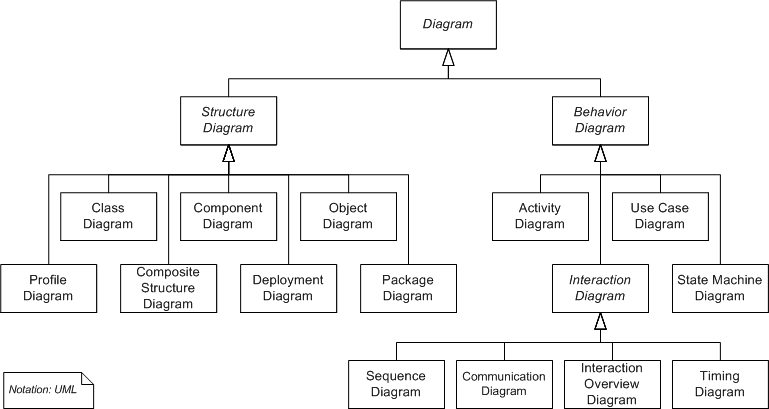
\includegraphics{img/umldiagram.png}
 \caption{UML-діаграма}
 \label{apdxfig:umldiagram}
\end{figure}

\end{a3paperl}

        % додаток другий
%!TEX root = ../bdr.tex

\acode{08-02}%
\bcode{БКР}%
\ccode{000}%
\dcode{13}%
\ecode{000}
\fcode{Е3}
\partdes{Схема електрична принципова}%


\begin{drawing}
\chapter[(Довідковий) Приклад додатку у форматі кресленика довга назва для перевірки перенесення]{}
\label{apdx:ozpsch}
% \begin{picture}(0,0)
%   \put(-105,-740.6){\frame{\hbox{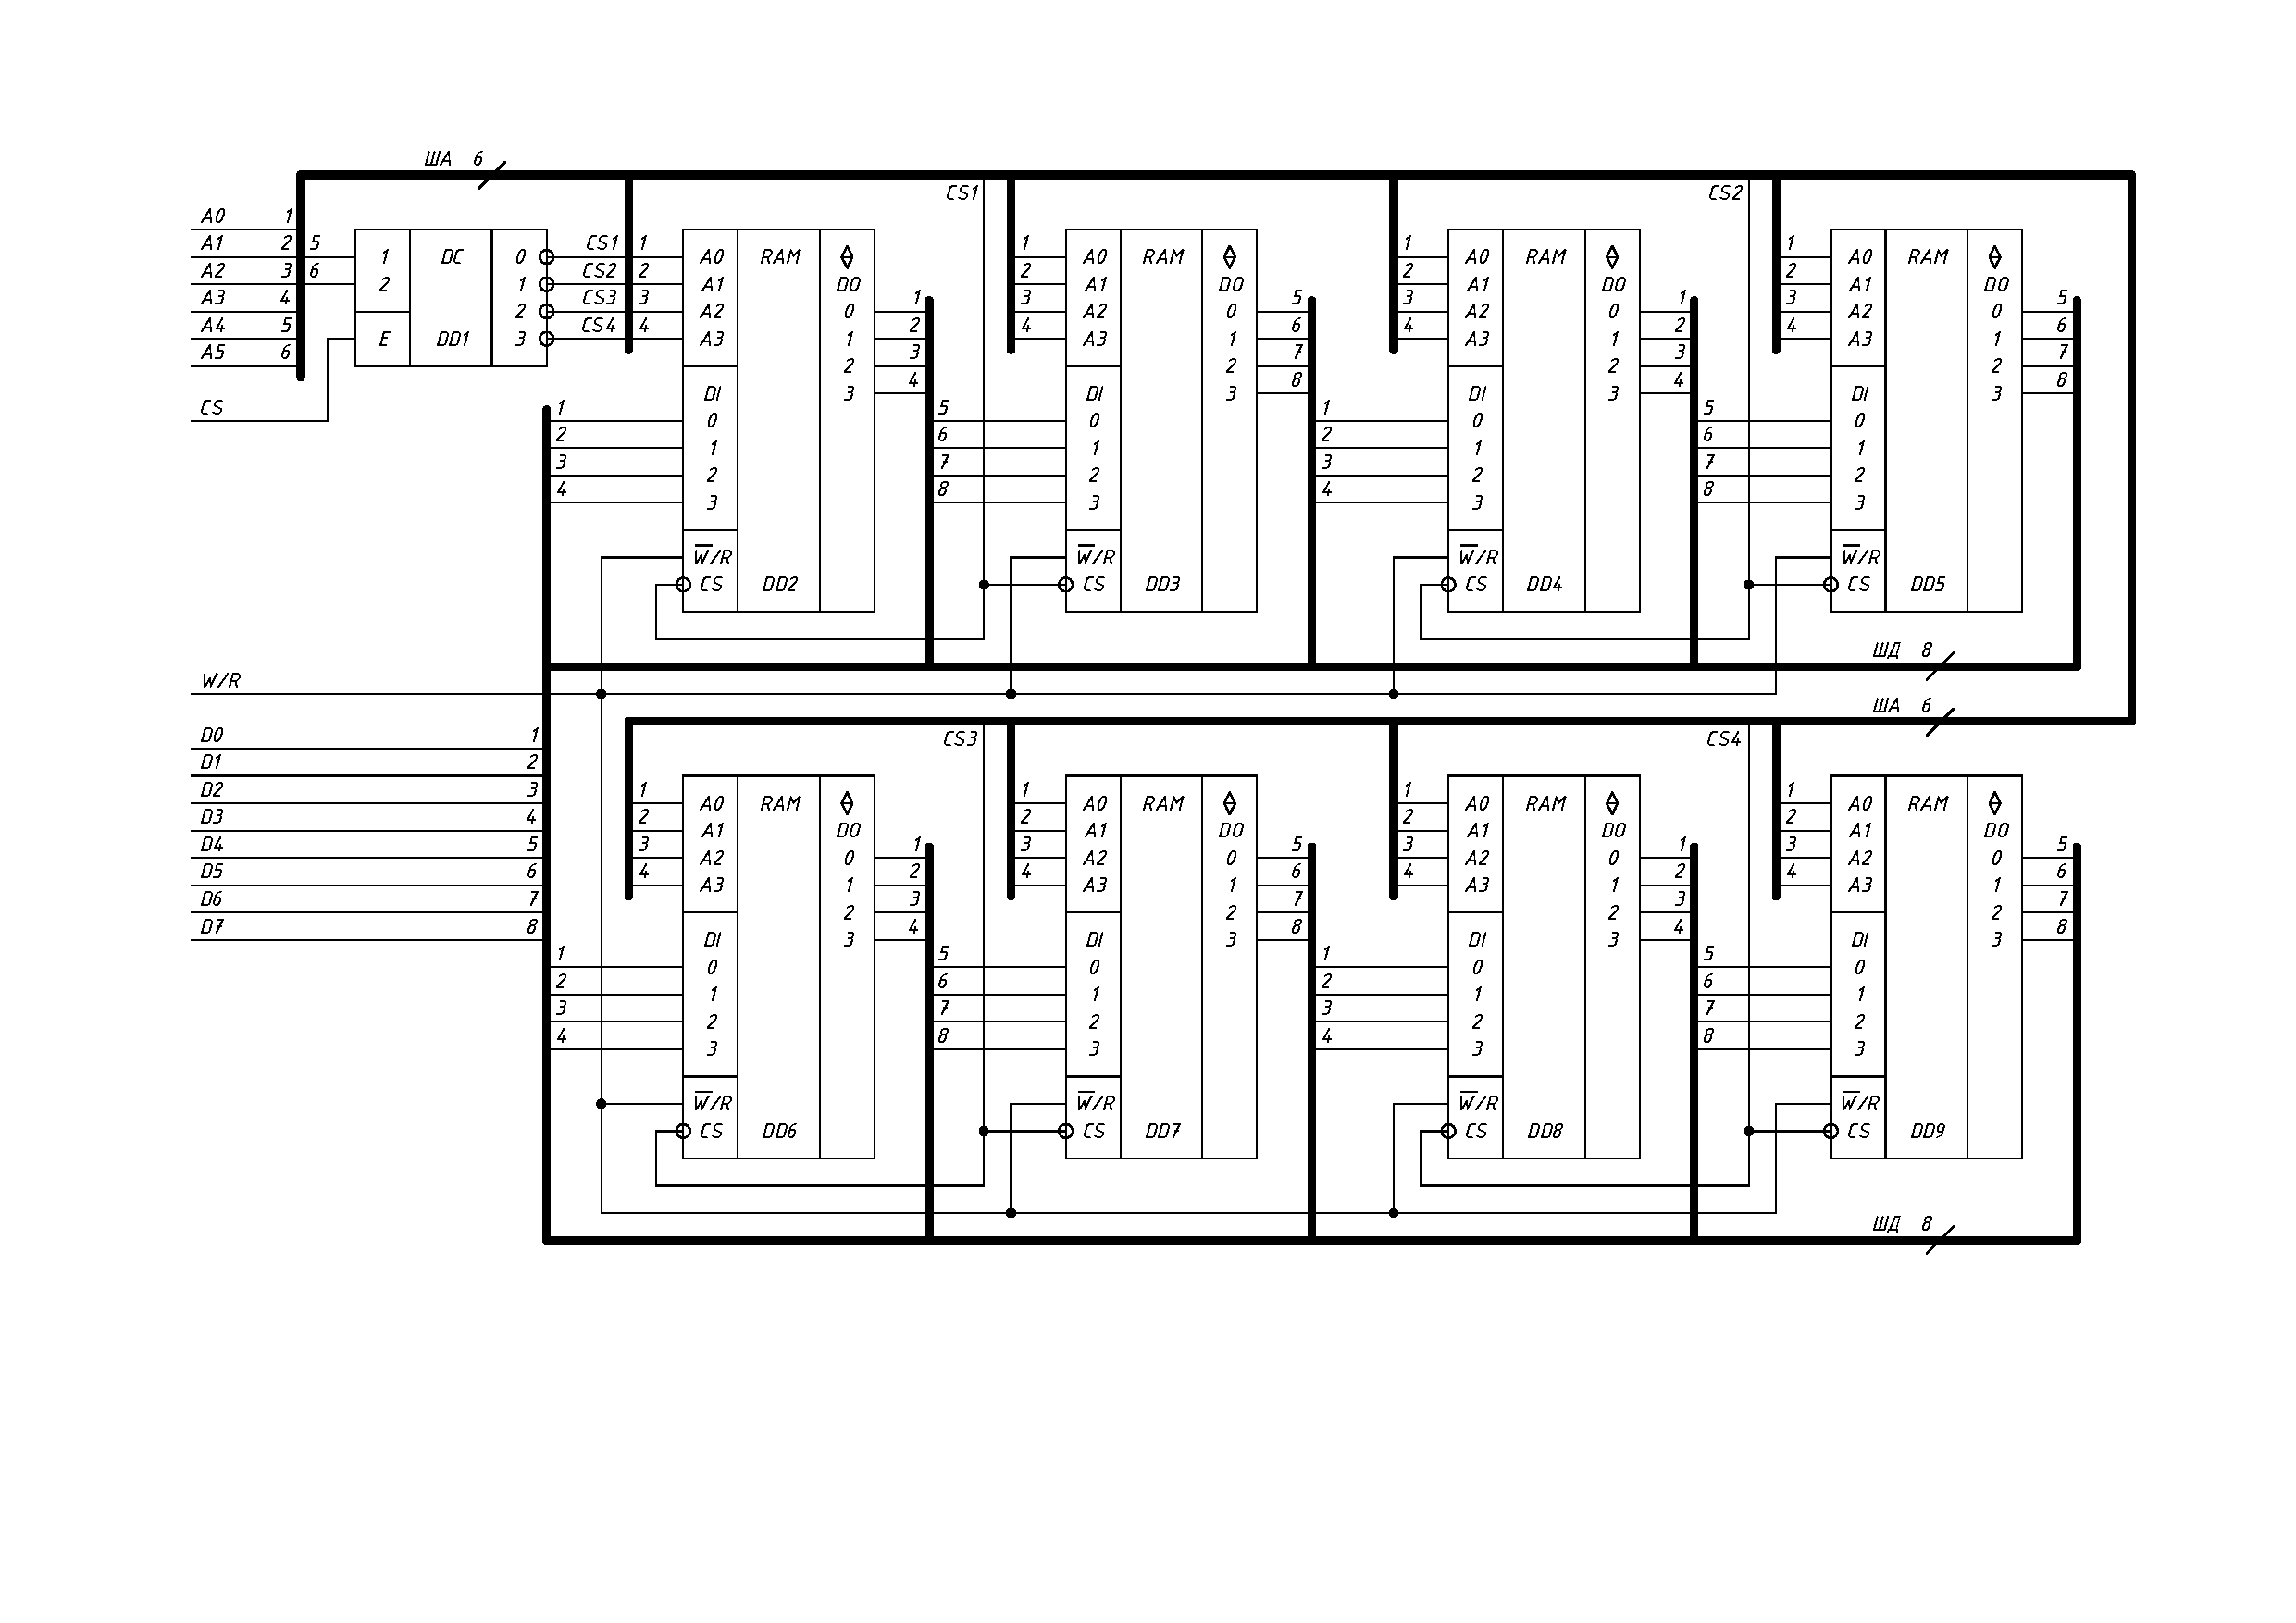
\includegraphics{img/sch4.pdf}}}}
% \end{picture}

\AddToHookNext{shipout/background}
   %{\put(0,-\paperheight){\frame{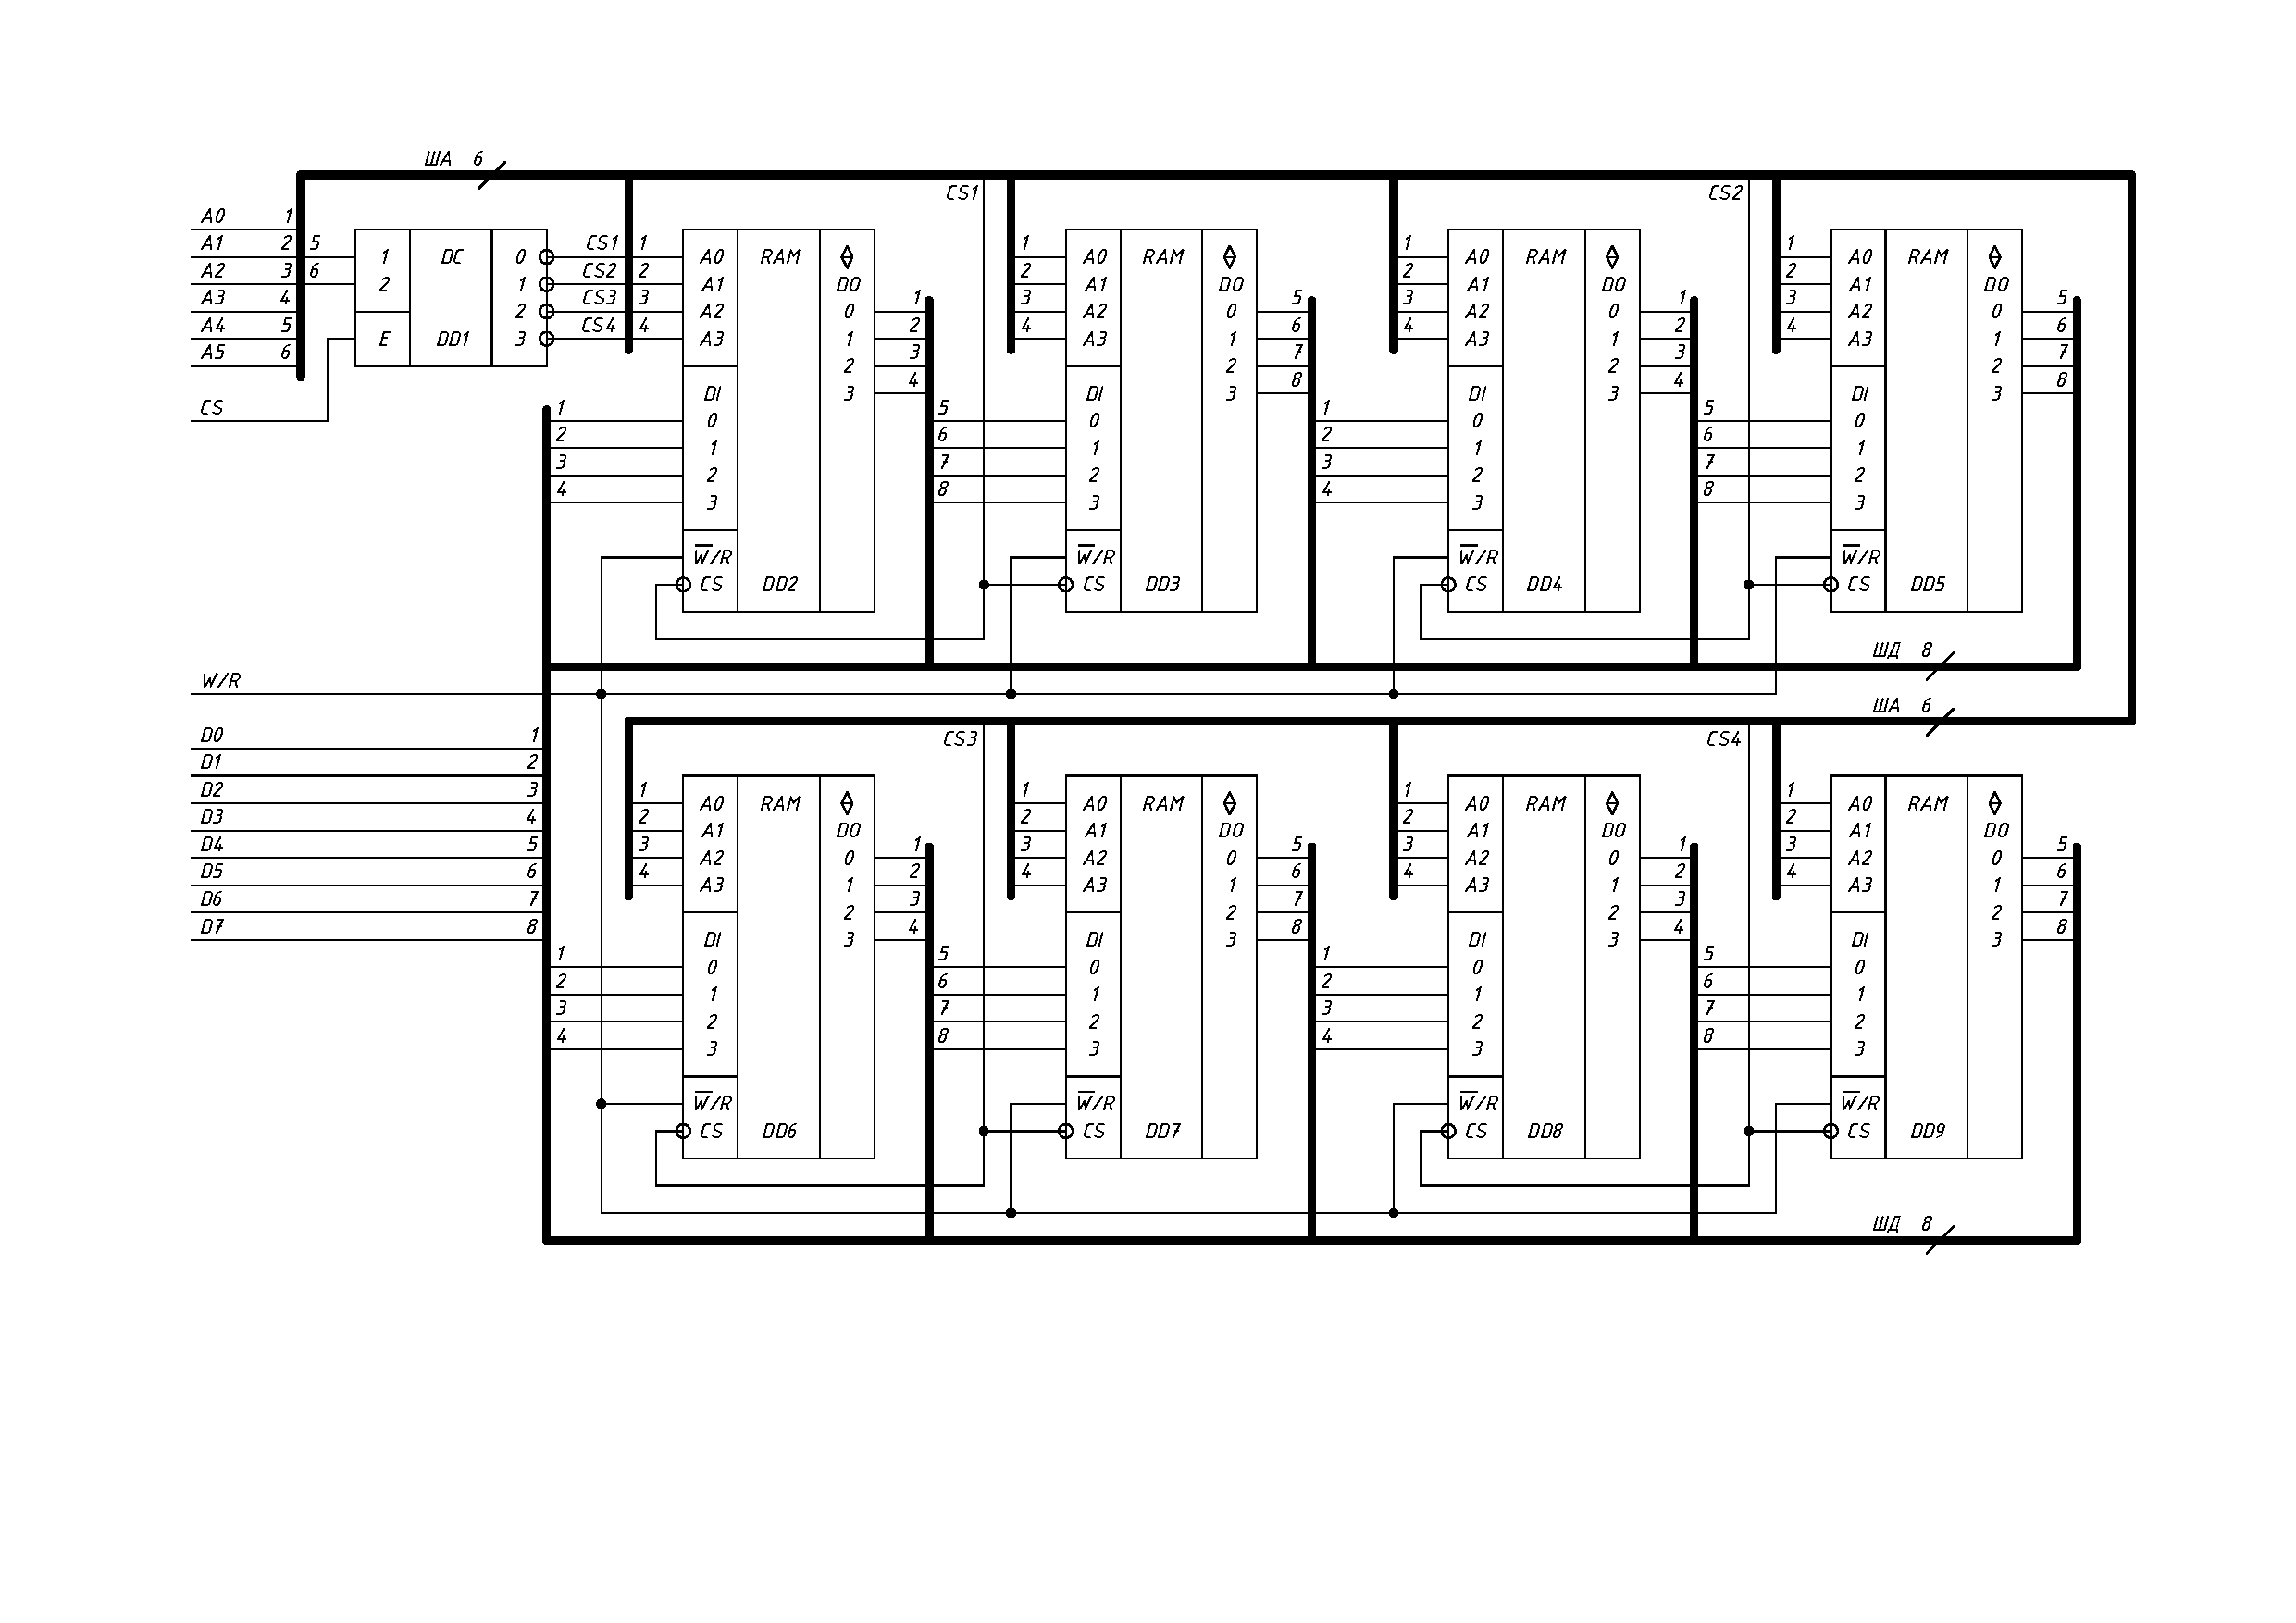
\includegraphics{img/sch4.pdf}}}}
   {\put(0,-\paperheight){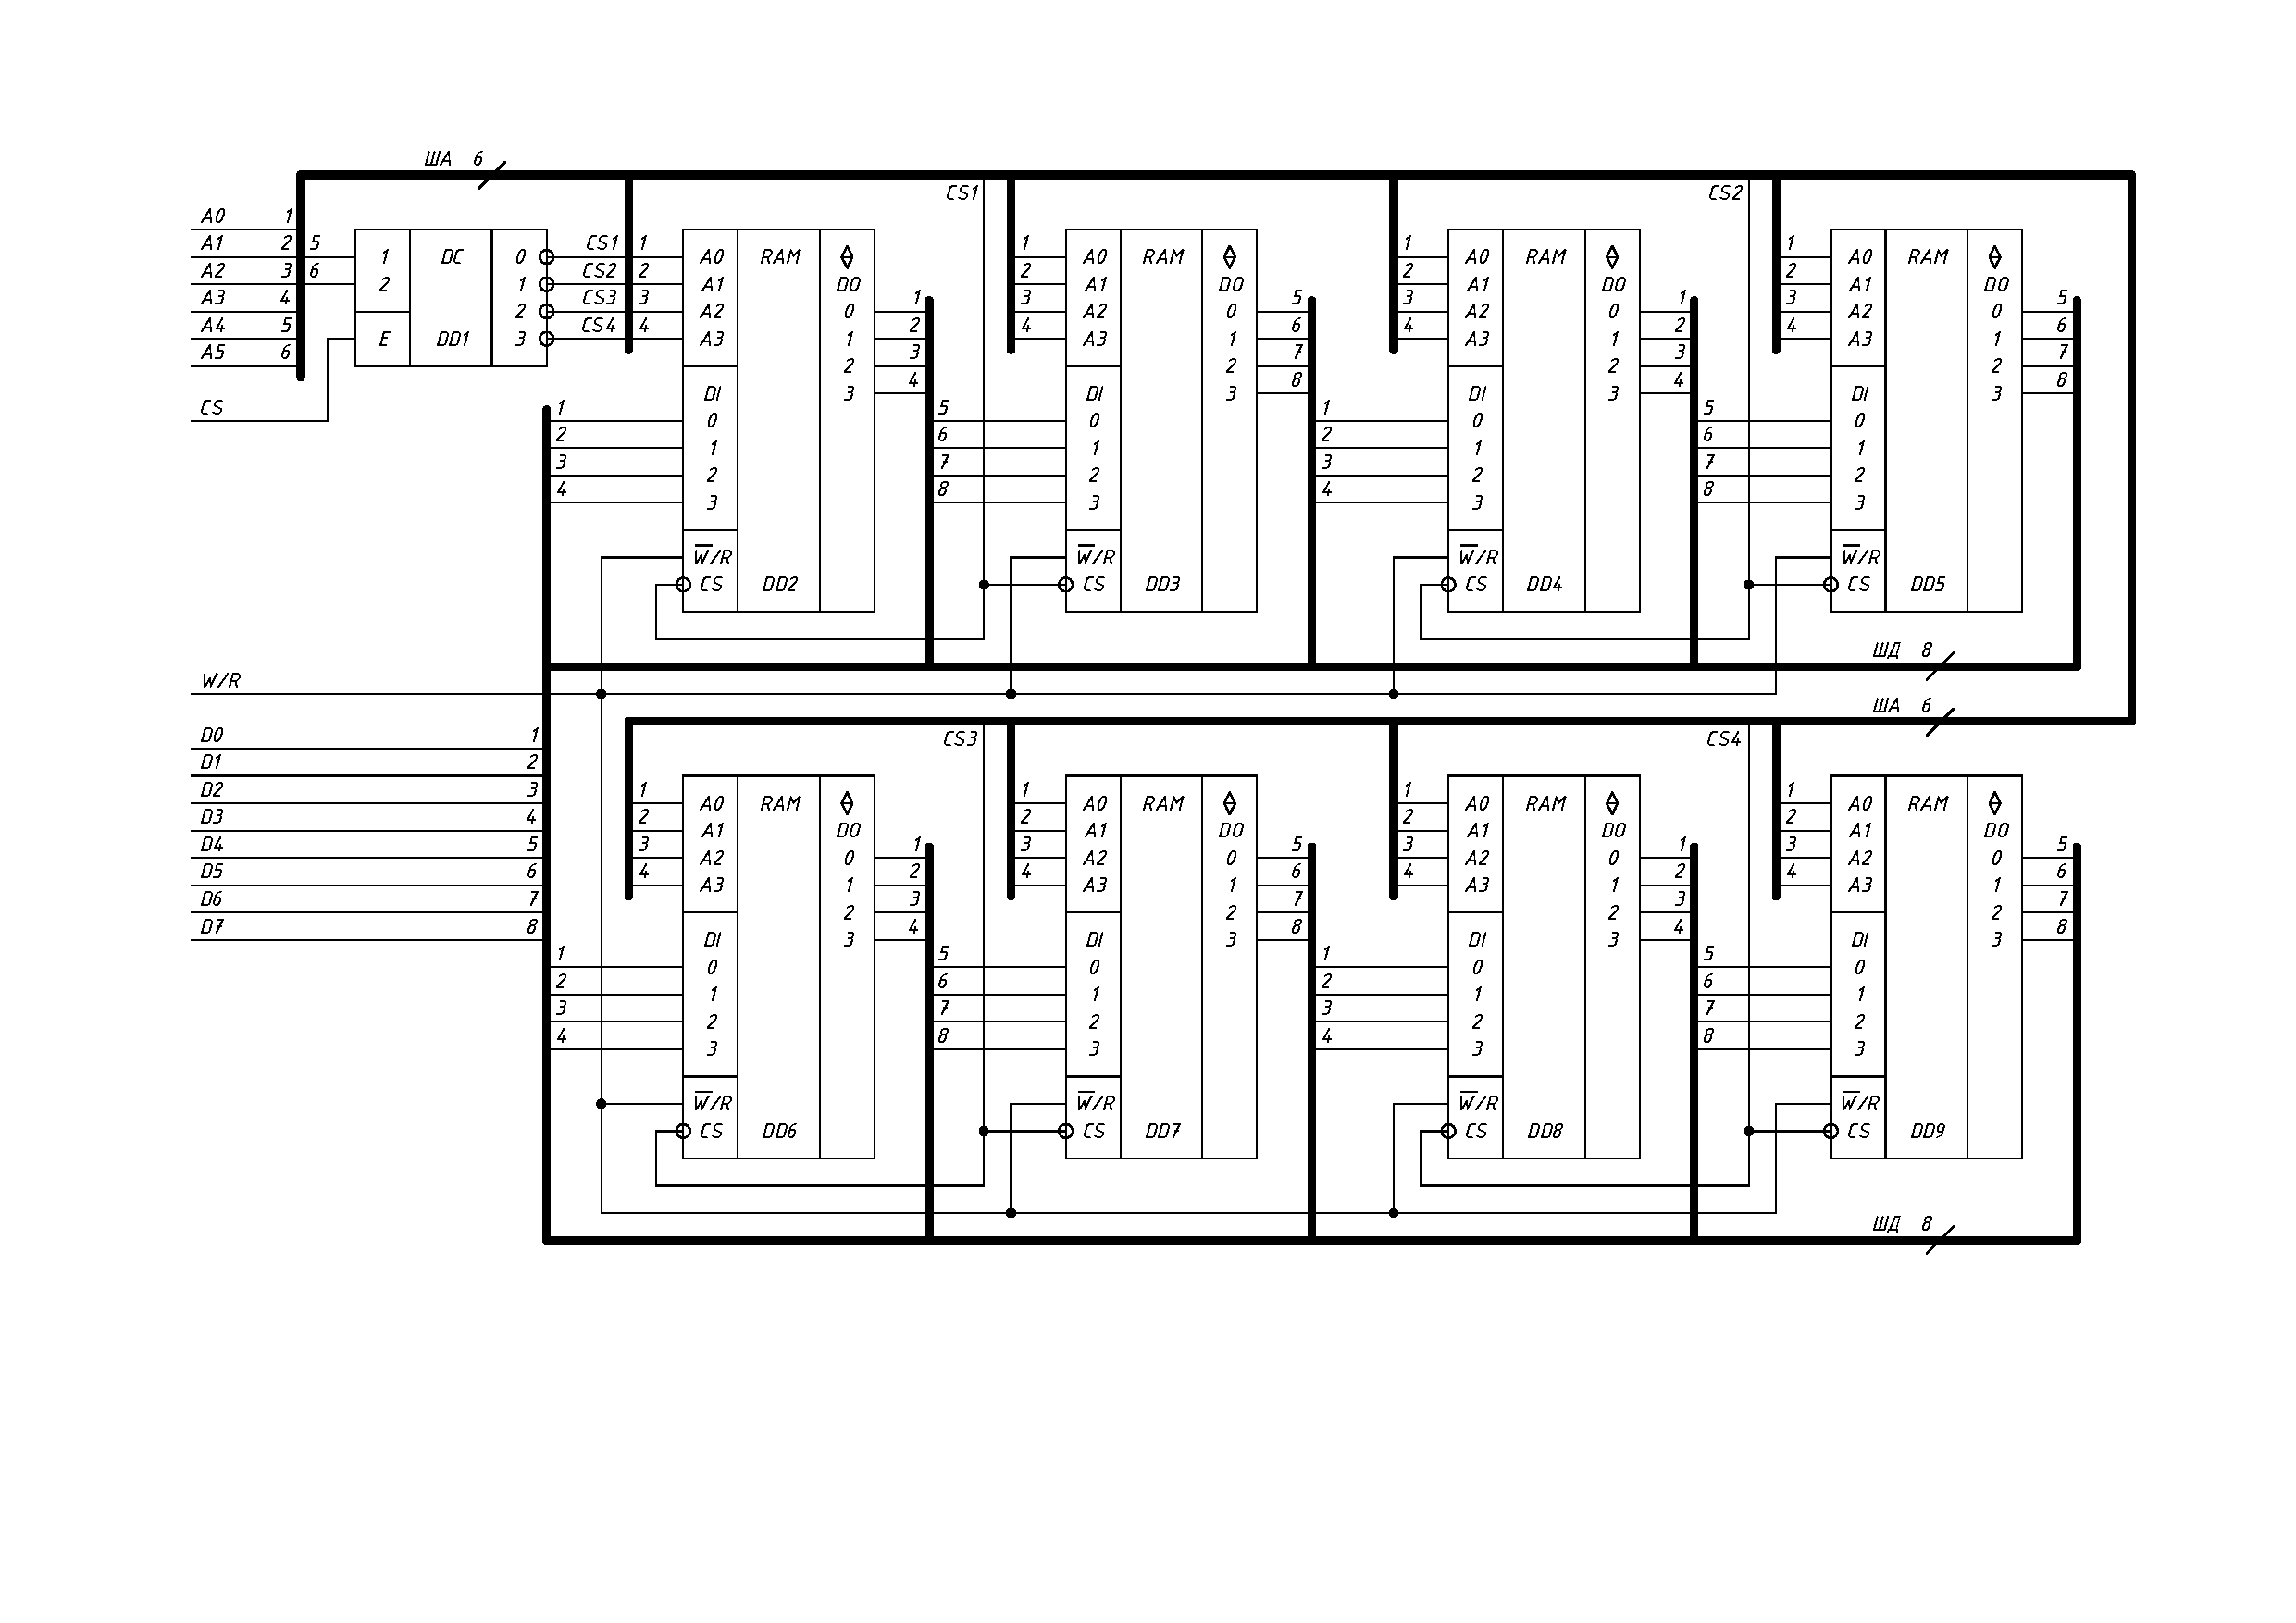
\includegraphics{img/sch4.pdf}}}
\end{drawing}
%\newgeometry{a4paper,left=3cm,top=2.0cm,bottom=2.5cm,right=1.5cm,layoutvoffset=0.5cm}

     % додаток третій
%!TEX root = ../bdr.tex
\chapter[(Довідковий) Приклад вставки коду вручну через середовище minted]{Приклад вставки коду вручну через середовище minted}

\begin{minted}  % приклад вставки коду вручну через середовище minted 
[
frame=lines,
framesep=2mm,
baselinestretch=1.2,
fontsize=\footnotesize,
linenos
]
{python}
import numpy as np
    
def incmatrix(genl1,genl2):
    m = len(genl1)
    n = len(genl2)
    M = None #to become the incidence matrix
    VT = np.zeros((n*m,1), int)  #dummy variable
    
    #compute the bitwise xor matrix
    M1 = bitxormatrix(genl1)
    M2 = np.triu(bitxormatrix(genl2),1) 

    for i in range(m-1):
        for j in range(i+1, m):
            [r,c] = np.where(M2 == M1[i,j])
            for k in range(len(r)):
                VT[(i)*n + r[k]] = 1;
                VT[(i)*n + c[k]] = 1;
                VT[(j)*n + r[k]] = 1;
                VT[(j)*n + c[k]] = 1;
                
                if M is None:
                    M = np.copy(VT)
                else:
                    M = np.concatenate((M, VT), 1)
                
                VT = np.zeros((n*m,1), int)
    
    return M
\end{minted}
    % додаток четвертий
\end{document}
